This chapter outlines some backtround theory that will be important throughout
the rest of the thesis. In section~\ref{theroy:cool} I will give an abstracted
overview of the principles of laser-cooling and trapping of atoms and
molecules, including magnetic traps. In section~\ref{theory:chips} I will
explain how it is possible to create magnetic fields for such traps using wires
on the surface of a chip. Finally, I will introduce the structure of diatomic
molecules, which is essential for applying these techniques in our experiment.

\section{Laser-cooling and trapping}

\subsection{Doppler cooling}

We will introduce Doppler cooling in the idealised case of a two-level atom or
molecule (henceforth the particle) travelling in one dimension, $x$.  Say that
light is incident on the particle from the positive $x$ direction. If the light
is resonant with an internal transition then the particle can absorb a photon,
which will at some later time be re-emitted the particle decays. The
emission of the photon has no preferred direction, and so over a large number
of these scatters the average effect is a net reduciton in the atom's velocity
in the positive $x$ direction.

In order to quantify this process, we might start by asking ourselves, what is
the force exerted on the particle by the photons? This will be~\cite{Foot2005}
%
\begin{equation}
  F = \text{photon momentum} \times \text{scattering rate}.
\end{equation}
%
The photon momentum is the usual value
%
\begin{equation}
  p_\gamma = \hbar k = \frac{hc}{\omega}
\end{equation}
%
and the scattering rate will be the product of the decay rate of the transition
(its linewidth) $\Gamma$ and the population of the excited state $\rho_{22}$.
We write the excited state in this way since it can be found from the optical
Bloch equations in the rotating wave approximation and in steady state to
be~\cite{Metcalf1999}
%
\begin{equation}
\rho_{22} = \frac{\Omega^2/4}{(\omega-\omega_0)^2 + \Omega^2/2 + \Gamma^2/4}.
\end{equation}
%
Where $\Omega$ is the Rabi frequency. We introudce the unitless parameters
$\delta = (\omega - \omega_0)/\Gamma$ and $s=\Omega^2/(2\Gamma)$ so that
%
\begin{equation}
  \rho_{22} = \frac{s/2}{\delta^2 + 1 + s}.
\end{equation}
%
We can now write down the scattering rate
%
\begin{equation}
  R = \frac{s\gamma}{\delta^2 + 1 + s}
\end{equation}
%
and force follows as
%
\begin{equation}
  F = \frac{s\gamma}{\delta^2 + 1 + s}\hbar k.
\end{equation}

The force acting on the particle can be related to its velocity by the Doppler
effect. A particle moving at speed $v$ will have its resonant frequency shifted
so that it has some new frequency $\omega'$ such that
%
\begin{equation}
  \frac{\omega'-\omega_0}{\omega_0} = \frac{v}{c},
\end{equation}
%
i.e.\ the frequency is red-detuned from the transition frequency at rest. The
result is that $\delta$ can be re-written as
%
\begin{equation}
  \delta \rightarrow \delta_+ = \delta + \frac{\omega_0}{\gamma c}v
\end{equation}
%
where $\delta$ represents the detuning of the laser from the resonant frequency
at rest, and the second term is the additional shift due to the Doppler effect.

However, what if the light is incident from the negative $x$ direction? In this
case, there is a blue shift, and we have
%
\begin{equation}
  \delta \rightarrow \delta_- = \delta - \frac{\omega_0}{\gamma c}v.
\end{equation}
%
By combining counter-propagating beams, it is possible to create a net force
%
\begin{equation}
  F_\text{res} = F_+ + F_-
\end{equation}
%
where
%
\begin{equation}
  F_\pm = \frac{s\gamma}{\delta_\pm^2 + 1 + s}\hbar k.
\end{equation}
%
For small $v$ we perform a Taylor expansion around $v=0$ to find that
%
\begin{equation}
  F_\text{res} \approx \frac{ s \delta}{(1 + s
  +\delta^2)^2}4\hbar k^2v.
\end{equation}
%
Which is maximised when $\delta = -1$ and $s = 1 + \delta^2 = 2$, so that
%
\begin{equation}
  F = - \alpha v
\end{equation}
%
where $\alpha  = - \hbar k^2 /2$.

So the counter-propagating beams provide a velocity-dependent damping
force. We call this arrangement an optical molasses, and it can equally be
applied in three dimensions.
%
It is important to note that the particles will not be brought to a standstill
under this effect. The molasses force does not contain the information
on the heating that occurs when the particles re-emit the absorbed photons.
This stochastic process limits the minimum attainable temperature to the
Doppler temperature~\cite{Metcalf1999}
%
\begin{equation}
  T_D = \frac{\hbar\Gamma}{k_B}.
\end{equation}

\subsection{Magneto-optical trap}

Doppler cooling is an important tool in the creation of ultracold atoms and
molecules, but it is of note that this technique does not provide any
position-dependent restoring force. In other words, particles that are slowed
by the above-described techniques are not trapped.
%
The magneto-optical trap (MOT) is the preeminent tool of atomic and molecular
physics, providing a way to trap a relatively cold gas of particles. It is the
backbone of many experiments including our own~\cite{Williams2017}. In this
section I will describe the basic operation of the common type-I MOT, that is a
two level system where the ground state has angular momentum $F$ and the
excited state has angular momentum $F'$ such that $F''>F$. In this example
$F=0$ and $F'=1$ are chosen.  In reality the molecule MOT that we will discuss
is a type-II MOT ($F'\leq F$) but such systems are more complicated and will be
discussed in the context of our experiment in section~\ref{section:overview}.

The MOT consists of two components, a magnetic quadrupole field, and restoring
laser beams, which are detuned from the $F\rightarrow F'$ transition by some
amount $\delta$. This setup is shown for one dimension in
\myfigref{theory:fig:MOT}. The Zeeman effect lifts the degeneracy of the excited state, and
introudces the usual energy shift~\cite{Binney}
%
\begin{equation}
  \Delta E = g_F m_F \mu_B B
  \label{theory:eqn:zeeman}
\end{equation}
%
where $g_F$ is the Land\'e g-factor, $\mu_B$ is the Bohr magneton, and $B$ is
the magnetic field. For a one-dimensional quadrupole field, we write $B=B'x$,
where $B'$ is the field gradient. We therefore have a position-dependent change
in the energy. Note that for negative $x$, the $m_F=-1$ state has lower energy,
and for positive $x$ the $m_F=1$ state has lower energy (when $g_F>0$, if
$g_F<0$ this is reversed).
%
The detuning $\delta$ is chosen such that this shift brings the lowered state
into resonance with the light. That the particle will then preferentially
absorb photons when it is away from the trap centre.

\begin{figure}[ht]
  \centering
  \includegraphics[width=0.8\textwidth]{figs/theory/motThesis.pdf}
  \caption{Illustration of the operating principle of a one-dimensional MOT on
    a two-level system with $F=0$ and $F'=1$. The particle is represented by
    the circle, and has counter-propagating beams of light (pink arrows)
    incident on it. A quardupole magnetic field is applied, lifting the
    degeneracy of the excited state as shown by the black lines. The light is
    red-detuned so as to be resonant with the transition to the lower $m_F$
    state, but only the restoring beam will be absorbed due to the choice of
    polarisation. The direction of the momentum change $\Delta\mathbf{p}$ is
    indicated by the black arrows. The excited state will decay back to the
    ground state (dashed lines).
  }
  \label{theory:fig:MOT}
\end{figure}

We wish to ensure that when a photon is absorbed the momentum change provides a
restoring force towards the centre of the MOT. This is achieved by choosing the
polarisation  so that the light coming from the positive (negative) direction
has $\sigma^+$ ($\sigma^-$) polarisation. The result is
that the particle will then always absorb light that is propagating towards the
centre of the trap, resulting in a restoring force. We also observe the same
Doppler cooling force from the molasses, so the resulting force is
%
\begin{equation}
  F = - \alpha v - \left(\frac{\mu_B B'}{\hbar k}\right)\alpha x.
\end{equation}

\subsection{Sub-Doppler cooling}

We might expect that a MOT would cool the atoms to around the Doppler
temperature, but in fact the temperate reached is often lower, due to
sub-Doppler cooling effects that often occur in a MOT. The most common of these
is polarisation gradient cooling, which cannot occur in the $F=0$, $F'=1$
system used to introduce the MOT. We instead consider a new system with
$F=1/2$, $F'=3/2$ which we note is still a type-I MOT.

In the centre of the MOT where there is near zero magnetic field, the $m_F$
states of the system would be degenerate expect that the degeneracy can be
lifted by the field of the light. This is the a.c. Stark shift, which is a
function of the light's polarisation. When the light has $\sigma_\pm$
polarisation, the $m_F=\mp1/2$ state is mixed more strongly with the exited
state, and so is higher. The relative matrix elements are shown in
\mysubfigref{theory:fig:subdoppler}{a}.

\begin{figure}[htb]
  \centering
  \begin{subfigure}[b]{0.45\textwidth}
      \cm{Optical pumping fig}
    \end{subfigure}
  \begin{subfigure}[b]{0.45\textwidth}
    \begin{overpic}[width=0.8\textwidth]{figs/theory/molasses.pdf}
      \put(4, 50){(b)}
      \put(105, 60){$F'=3/2$}
      \put(105, 28){$F=1/2$}
      \put(98, 2){Polarisation} % Was at x=105 but went outside hbox
    \end{overpic}
    \end{subfigure}
    \caption{In (a) we have \cm{some coupling matrix elements} Subfigure (b)
      shows the polarisation gradient cooling scheme described in the main
      text.  The polarisation gradient is depicted in the bottom row, and the
      $m_F=1/2$ ($m_F=-1/2$) state is shown by the dashed (solid) line. A
      particle in the molasses (pink circle) will follow a path such as the one
      shown here in pink, being pumped into the $F'=3/2$ state at the top of
      the potential hill, then decaying (dashed grey lines) back to the lower
      of the ground states and climbing the hill again.
  }
  \label{theory:fig:subdoppler}
\end{figure}

The counter-propagating beams establish a polarisation gradient across the
trap, and hence the Stark shift of the ground states also varies across the
trap, as shown in \mysubfigref{theory:fig:subdoppler}{b}. We have the additional effect that the
$m_F=\pm1/2$ state is only pumped by the $\sigma^\mp$ light, and so it happens
that the state with higher energy is the one that is excited. The excited state
can decay into the lower of the two ground states, where it will follow the
potential curve until it is pumped again. The particles on average spend more
time climbing the potential than descending it, and therefore expend energy
through this process, reducing their temperature to the recoil limit, which
corresponds to the energy exchanged by a single photon scatter
%
\begin{equation}
  T_\text{recoil} = \frac{\hbar^2 k^2}{m k_B}
\end{equation}
%
which is normally on the order of a \SI{1}{\micro\kelvin}.  Normally to achieve
such low temperatures the MOT field is switched off, so that only the molasses
is active, and the polarisation gradient cooling occurs across the entire
cloud.Lower temperatures can be reached by other techniques such as evaporative
cooling~\cite{Metcalf1999}.


\subsection{Magnetic trapping}
\label{theory:magtraps}

The MOT is an important tool for trapping, and can be configured in various
ways~\cite{Cotter2016, Lee:96, PhysRevLett.59.2631}, but there is considerable
benefit to being able to confine particles using only a magnetic field. Since
there is no light involved, it is much easier to control the trapping
potential. This opens the door to applications in
guiding~\cite{PhysRevLett.83.5194} and transporting~\cite{Nakagawa2005}
particles, but also confining close to a surface such as that of a chip. This will be
discussed in more detail in the next section, but for the moment we limit
ourselves to a basic description of magnetic trapping.

Continuing with the above example of a two-level particle with $F=1/2$,
$F'=3/2$, we notice that when the particle is in a state where $g_F m_F > 0$,
the Zeeman shift due to a magnetic field is positive (c.f.\
\myeqref{theory:eqn:zeeman}). Hence if the magnetic field $B$ is chosen such
that there is a local minimum in the vicinity of the particle, then these
states will be attracted to that minimum. Such a state is called a weak-field
seeker. We can equally have stong-field seeksers when $g_F m_F < 0$, but these
cannot be trapped since it is not possible to create a local magnetic field
maximum in free space.
%
Note that the dependence here is on the magnitude of the magnetic field, so the
direction of the field does not directly affect the trapping potential.

To magnetically trap our particle we need to first ensure it is in a
weak-field seeking state, and then we need to introduce a magnetic field with a
local minimum. It is possible to transfer into either of the states
$\ket{F=3/2, m_F=\pm3/2}$ by applying only $\sigma_\pm$ light to optically pump
into the respective state, as was discussed for sub-Doppler cooling. After the pumping scheme it is possible (if desired)
to transfer to either of the $\ket{F=1/2, m_F=\pm1/2}$ states by applying a
microwave pulse~\cite{WilliamsMagnetic2018}. Depending on the sign of $g_F$ (or for the excited state $g_{F'}$) 
one of these states is bound to be a weak-field seeker.

Now the final ingredient is a magnetic potential with a local minimum. There
are a plethora of examples to choose from, but the canonical choice is the
quadrupole trap, which can be fomred from a pair of anti-Helmholtz coils, as
shown in \mysubfigref{theory:fig:fields}{a}. We can approximate the field
generated near the centre of such a configuration as~\cite{Metcalf1999}
%
% TODO I use this equation somewhere else and I need to change to reference
% this one...
\begin{equation}
  \mathbf{B} = B'\begin{pmatrix} -x/2 \\ -y/2 \\ z \end{pmatrix}
  \label{theory:eqn:quadrupole}
\end{equation}
%
where $B'$ is the field gradient in the $z$ direction, and depends on the
currents in the coils as well as their geometry.

\begin{figure}
  \centering
  \includegraphics[width=0.7\textwidth]{figs/theory/QPIP.pdf}
  \caption{Subfigure (a) demonstrates the generation of a quadrupole field
    (pink arrows) by
  anti-Helmholtz coils (black arrows). Subfigure(b) demonstrates the current
  configuration for a
  Ioffe-Pritchard trap, with longitudinal currents (blue arrows) and endcap
coils (black arrows) The field near the trap centre is also shown (pink arrow).
\cm{reproduced from Ed's notes}}
  \label{theory:fig:fields}
\end{figure}

One of the drawbacks to a quadrupole is that the magnetic field at the centre
is zero. In regions of low field there is no breaking of the degeneracy, and so
it is possible for the $m_F$ quantum number to change to an un-trappable state.
This is known as a spin-flip or Majorana loss~\cite{Brink2006}. One method of
resolving this is to instead use a Ioffe-Pritchard trap, which has a non-zero
field minimum. The standard method of implementing such a trap is shown in
\mysubfigref{theory:fig:fields}{b}. Four straight wires are arranged in a
square, with a pair of parallel coils on either end to form end-caps. The field
generated is of the form
%
\begin{equation}
  \mathbf{B} = b_1 \begin{pmatrix} x \\ -y \\ 0 \end{pmatrix}
  + b_0 \begin{pmatrix} 0 \\ 0 \\ 1 \end{pmatrix}
  + b_2 \begin{pmatrix} -xz \\ -yz \\ z^2 - \rho^2/2 \end{pmatrix}
  \label{theory:eqn:IP}
\end{equation}
%
where $\rho^2 = x^2 + y^2$ and the constants $b_i$ are again functions
of the currents and the geometry.

For a quadrupole field, the motion is characterised by the gradient, but for a
Ioffe-Pritchard trap, the motion is harmonic, and we can find the frequencies
by evaluating the shape of the potential $\mu B$, where $\mu$ is the magnetic
moment of the trapped state. From \myeqref{theory:eqn:IP} we have
%
\begin{equation}
  \mu B \approx \mu \sqrt{b_0^2 + (b_1^2 -
  b_0b_2)\rho^2 + 2b_0b_2z^2}.
\end{equation}
%
Up to the third order in position terms. Now expanding for $z=0$ and small $\rho$ we get
%
\begin{equation}
  \mu B \approx \mu b_0\left(1 + \frac{b_1^2 -
    b_0b_2}{2b_0}\rho^2\right)
\end{equation}
%
which is a harmonic potential with minimum $\mu b_0$ and frequency
%
\begin{equation}
  \omega_\rho = \sqrt{\frac{\mu}{m}\left(\frac{b_1^2}{b_0}-b_2\right)}
\end{equation}
%
for a particle of mass $m$.

Similarly for the $z$ direction, we can find the potential
approximates to
%
\begin{equation}
  \mu B = \mu b_0 (1 + b_2 z^2)
\end{equation}
%
which is again harmonic, with frequency
%
\begin{equation}
  \omega_z \approx \sqrt{\frac{\mu}{m}2b_2}.
\end{equation}

We note that the motion of the particles in the trap must be slow compared to
the resonant frequency $g_F\mu_BB/\hbar$ to avoid inducing transitions.
Similarly, the field can be changed adiabatically (slowly compared to the speed
of the trapped particles) without heating. This can be used for
transport, or transferring particles between magnetic traps, and will be
discussed further in chapter~\ref{sim}.

\section{Chip trap theory}
\label{theory:chips}

The main subject of this thesis is the trapping of particles near chips. In
this section we will see that it is possible to use wires on a chip, combined
with external magnetic fields to produce trapping potentials that resemble
either a quadrupole or Ioffe-Pritchard trap. Further details can be found in
\inlineref{2011Ac}.

\subsection{Simple wire traps}

We begin our discussion by considering a simple case of a two-dimensional trap.
This will be formed of a straight wire carrying current $I$, which we
approximate to have infinite length. Such a wire can be free-standing or
deposited on a substrate. The magnetic field due to the wire is described by
the Biot-Savart law, having magnitude
%
\begin{equation}
  B_w(r) = \frac{\mu_0 I}{2 \pi r}
\end{equation}
%
where $r$ is the distance from the wire. The direction of the field obeys the
right hand rule. With such a geometry it is possible to create a rudimentary
two-dimensional trap at a distance $h$ from the wire, by applying an external
bias field $\mathbf{\tilde{B}}$, whose direction opposes the field of the wire.
To create the trap at the desired bias, the strength of the field must be
$\tilde{B}_y = B(h)$.

%TODO Use this notation in sim when descirbing calculation of the field!
Figure \myfigref{theory:fig:simplefield} illustrates this two-dimensional trap.
Here the wire oriented along the $x$ direction, with the current
$I=\SI{1}{\milli\ampere}$, flowing in the
positive direction (out of the page). This generates the expected field
$\mathbf{B}$ shown in subfigure (a). This is superimposed with the bias field
$\mathbf{\tilde{B}}_y$, also shown in (a), to produce the resulting field
$\mathbf{B} = \mathbf{B}_w + \mathbf{\tilde{B}}$ shown
in (b). This subfigure details the field lines (pink arrows) and field
magnitude, shown by the colour gradient
(blue, guide to the eye) where darker areas indicate lower field. The bias field
is chosen to induce a field minimum at $h=\SI{1}{\milli\meter}$. Subfigure (c)
shows a cut through of the potential along $y$ with $x=0$, $z=h$. Subfigure (d)
also shows a cut through of the potential along $z$ with $x=y=0$. This
demonstrates the two-dimensional trap.

\begin{figure}[htbp]
  \centering
  \begin{subfigure}[b]{0.45\textwidth}
    \centering
    \hfill{}
    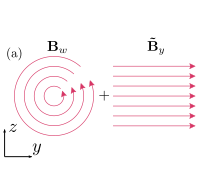
\includegraphics[width=0.8\textwidth]{figs/theory/wires/simplefield.pdf}
    \hfill{}
  \end{subfigure}
  \begin{subfigure}[b]{0.45\textwidth}
    \centering
    \import{figs/theory/wires/}{simpleheat_alone.pgf}
  \end{subfigure} \\
  \begin{subfigure}[b]{0.45\textwidth}
    \centering
    \import{figs/theory/wires/}{simpleheat_y.pgf}
  \end{subfigure}
  \begin{subfigure}[b]{0.45\textwidth}
    \centering
    \import{figs/theory/wires/}{simpleheat_z.pgf}
  \end{subfigure}
  \caption{
    The field from a simple two-dimensional wire trap. In subfigure (a) a wire carries
    current $I=\SI{1}{\milli\ampere}$ in the positive $x$ direction (out of the
    page) to create the usual field $\mathbf{B}_w$. This is combined with the
    external bias field $\mathbf{\tilde{B}}_y$ to create the two-dimensional trap
    at height $h=\SI{1}{\milli\meter}$
    shown in subfigure (b). The field lines are shown by pink arrows, and the
    magnitude of the resulting field is shown with the blue gradient (darker
    means weaker field, guide to the eye). Cut throughs of the potential are
    shown for $y$ (with $x=0$, $z=h$) in (c) and for $z$ (with $x = y = 0$) in
    (d).
  }
  \label{theory:fig:simplefield}
\end{figure}

Since the field minimum here is a zero, we can approximate the value near the
centre by a (two-dimensional) quadrupole with gradient
%
\begin{equation}
  B' = -\frac{2\pi \tilde{B}_y^2}{\mu_0 I}.
\end{equation}
%
The depth of the trap is $\mu \tilde{B}_y$, where $\mu$ is the magnetic dipole
moment of the trapped particle. This can be seen in
\mysubfigref{theory:fig:simplefield}{d}: the potential is $B = |B_w(z) +
\tilde{B}_y|$, and so has an asymptote at $B=|\tilde{B}_y|$ as
$z\rightarrow\infty$. We usually write this depth as a temperature
%
\begin{equation}
  T  = \frac{\mu \tilde{B}_y}{k_B}.
  \label{theory:eqn:depth}
\end{equation}
%
We can transform such a trap into a Ioffe-Pritchard trap by applying a second
bias field along the $x$ direction to lift the field minimum away from
zero.

Of course, it is commonly desirable to trap in all three dimensions. A simple
way to introduce confinement along the $x$ axis is to introduce a second wire
trap acting in the perpendicular direction. Such a device is called a dimple
trap (or cross conductor trap, or X-trap) and is illustrated in
\myfigref{theory:fig:dimple}. We label the current in the second wire $I_1$
and the new bias field, which is parallel to the $x$-axis and opposes the
$I_1$ field is labelled $\mathbf{B}_x$. In the case that $I_1 \ll I$, the
second wire can be treated as a perturbation of the first. The field minimum is
therefore still at $h$, and its depth is given by \myeqref{theory:eqn:depth}.

\begin{figure}[htb]
    \centering
    \begin{tabular}[t]{cc}
\begin{subfigure}{0.3\textwidth}
    \centering
    \smallskip
    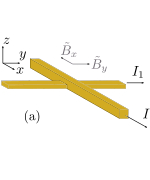
\includegraphics[width=\textwidth]{figs/theory/wires/dimple.pdf}
\end{subfigure}
    &
        \begin{tabular}{c}% if you add [t], than sub images are pushed down
        \smallskip
            \begin{subfigure}[t]{0.4\textwidth}
                \centering
                  \import{figs/theory/wires/}{dimpleheat_alone.pgf}
            \end{subfigure}\\
            \begin{subfigure}[t]{0.4\textwidth}
                \centering
                  \import{figs/theory/wires/}{dimple_x.pgf}
            \end{subfigure}
        \end{tabular}\\
    \end{tabular}
  \caption{
    The geometry of the dimple trap is shown in subfigure (a), with the new
    wire along $y$ carrying current $I_1$ intersecting the $I$ wire. An
    additional bias field in the $x$ direction, $\tilde{B}_x$ creates the field
    minimum. The field lines (pink) and magnitude (blue, darker is weaker,
    guide to the eye) is shown in subfigure (b) along $x=0$. Note the strong
    field region along the $y$ axis around the $I_1$ wire. Subfigure (c) shows
    a cut through of the trapping potential in the $x$ direction with $y=0$,
    $z=h$.
  }
  \label{theory:fig:dimple}
\end{figure}

The dimple trap can be used as a quadrupole trap when the bias fields are
chosen to exactly cancel the magnetic field at the centre, or it can be used as
a Ioffe-Pritchard trap when there is a non-zero minimum. We will focus on the
latter case, in which case it is useful to write down the trap frequencies, the
derivation of which is similar to the one for the six-wire field discussed in
section~\ref{theory:magtraps}.
%
Since the trapping from the $I$ wire will be stronger than the $x$-axis
confinement from the $I_1 << I$ wire, we $\omega_x$ to be the weak trapping
direction. We again write down the field minimum
%
\begin{equation}
  B_0 = \left|\tilde{B}_x + \frac{\mu_0 I_1}{2\pi h}\right|,
\end{equation}
%
the transverse gradient
%
\begin{equation}
  B'_\perp = \frac{\mu_0 I}{2 \pi h^2},
\end{equation}
%
and the curvature along the weak component
%
\begin{equation}
  B'' = \frac{\mu I_1}{\pi h^3}.
\end{equation}
%
The trap frequency in the strong direction is
%
\begin{equation}
  \omega_\perp = \sqrt{\frac{\mu B_\perp'^2}{m B_0}}
  \label{theory:eqn:perpfreq}
\end{equation}
%
where $m$ is the particle mass. In the weak direction (along $x$) the frequency
is
%
\begin{equation}
  \omega_x = \sqrt{\frac{\mu B''}{m}}.
  \label{theory:eqn:xfreq}
\end{equation}

\subsection{The H-trap}

Consider the dimple trap, but with $\tilde{B}_x$ set to zero. Now what was
previously a magnetic field minimum will be a field maximum. By putting two
such dimple traps next to each other, it is possible to create a local minimum
within which we can trap molecules. Such a trap is called an H-trap, and is
pictured in \myfigref{theory:fig:Htrap}. We label the current due to the second
dimple trap $I_2$, and again note that the bias field in the $x$ direction can
be set to zero. The distance between $I_1$ and $I_2$ is denoted $d$, and we now
refer to the wire carrying current $I$ as the axis of the trap.

\begin{figure}[htb]
  \centering
  \begin{subfigure}[b]{0.4\textwidth}
    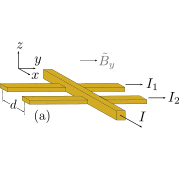
\includegraphics[width=\textwidth]{figs/theory/wires/Htrap.pdf}
    %\vspace{0.1mm}
  \end{subfigure}
  \begin{subfigure}[b]{0.4\textwidth}
    \import{figs/theory/wires/}{Hx.pgf}
  \end{subfigure}
  \caption{The geometry of the H-trap is shown in subfigure (a). In subfigure
  (b) we show the potential for an H-trap with
  $I_1=I_2=I/10=\SI{0.1}{\milli\ampere}$ and $d=\SI{10}{\milli\meter}$. Again the bias field is chosen so
  that $h=\SI{1}{\milli\meter}$.}
  \label{theory:fig:Htrap}
\end{figure}

We note that we need not choose $I_1$ and $I_2$ to be the same, although from
now on we will assume that they have the same magnitude, the sign can differ.
In other words these currents can be parallel or anti-parallel. In the former
case the trap forms a Ioffe-Pritchard trap; this is due to the fields from
$I_1$ and $I_2$ adding in the centre, to provide some overall non-zero
component in the $x$ direction. When the currents are anti-paraellel, the $I_1$
field opposes the $I_2$ field in the centre of the trap, the two cancel and
there is a field zero. Hence the latter configuration is a quadrupole trap.

In the Ioffe-Pritchard configuration, we can write down the field's
minimum
%
\begin{equation}
  B_0 = \tilde{B}_x + 2\tilde{B}_y \frac{I_1}{I}\frac{h^2}{(d/2)^2 + h^2}
\end{equation}
%
transverse gradient
%
\begin{equation}
  B'_\perp = \frac{2\pi\tilde{B}_y}{\mu_0 I}
\end{equation}
%
and curvature~\cite{PhysRevA.79.013407}
%
\begin{equation}
  B'' = \tilde{B}_x + 2\tilde{B}_y\frac{I_1}{I_0}\frac{h^2}{(d/2)^2+h^2}
\end{equation}
%
and the trap frequencies are again given by equations~\ref{theory:eqn:perpfreq}
and~\ref{theory:eqn:xfreq}~\cite{PhysRevA.79.013407}. In the quadrupole
configuration, the traps is characterised by the perpendicular gradient
$B'_\perp$. 

\subsection{Three dimensional single-wire traps}

Although the H-trap provides a method of creating a three dimensional
microtrap, it is not always convenient to have to use three distinct wires.
Fortunately the H-trap can be approximated by a single wire, either in a
U-shape for the quadrupole variant, or a Z-shape for the Ioffe-Pritchard
variant. These are pictured in \myfigref{theory:fig:HUZ}. Note that for the U-trap
the currents in the off-axis wires are once again anti-parallel, and in the
Z-trap these currents are parallel. For the U- and Z-traps, we denote the
distance between the end wires as $d$, and again refer to this as the axis.

\begin{figure}[htbp]
  \centering
  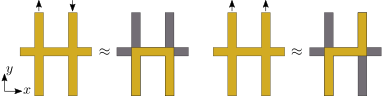
\includegraphics[width=\textwidth]{figs/theory/wires/HUZcomp.pdf}
  \caption{Current configuration for U-trap (Z-trap) approximating the
  quadrupole (Ioffe-Pritchard) H-trap configuration.}
  \label{theory:fig:HUZ}
\end{figure}

The Z-trap will be the primary focus of this thesis, and so we will focus on
this as an example. In \myfigref{theory:fig:HZcontours} we compare an H-trap
with a current of \SI{1}{\milli\ampere} on each wire with the potential due to
a single Z-wire also with current \SI{1}{\milli\ampere}. In both cases
$d=\SI{10}{\milli\meter}$, and a bias field of \SI{2}{\milli\gauss} in the $y$
direction is chosen, so as to create a minimum at approximately
$z=\SI{1}{\milli\meter}$ from the axis. The potentials are similarily
comparable for the H-trap in quadrupole configuration and the U-trap.

\begin{figure}[htbp]
  \centering
  \import{figs/theory/wires/}{HZcontours.pgf}
  \caption{Contour plots comparing the potentials for a H-trap in
    Ioffe-Pritchard configuration (left column) and Z-trap (right column), with
    cut throughs for $z=\SI{1}{\milli\meter}$ (top row) and $x=0$ (bottom row).
    All wires carry a current of $I=\SI{1}{\milli\ampere}$ and a bias field of
    \SI{2}{\milli\gauss} is applied in the $y$ direction.}
  \label{theory:fig:HZcontours}
\end{figure}

This illustrates that a single current-carrying wire can be used to form a trap
in three dimensions. The examples here use length scales of a few millimeters,
and have typical depths of \SI{100}{\nano\kelvin}, but we will discuss in
chapter~\ref{sim} that it is possible to realise much smaller trap and deeper
traps.


\section{Physics of diatomic molecules}
\label{theory:molecules}

Up to this point we have considered abstracted and idealised systems, but in
the next chapter we will begin to think about the realities of implementing a
cold molecule experiment. It is essential that we introduce and understand the
energy structure of diatomic molecules, which is far richer and more complex
than the structure of atoms, due to the additional effects of vibration and
rotation of the two nuclei. This section will explain the physics of diatomic
molecules so that the particulars of the cooling transitions and magnetically
trappable states can be easily explained in the next chapter. A far more
detailed review of the topic can be found in \inlineref{brown_carrington_2003}.

\subsection{Electronic, vibrational, and rotational energy}

We can begin by considering two atoms or ions, which we label $A$ and $B$,
with masses  $m_i = m_p Z_i$, $i\in\{A,B\}$ and $m_p$ is the proton rest mass. We say that the location of the
atoms is $\mathbf{R}_i$ and the distance between them is
$R_{AB}$ where $\mathbf{R}_{AB} = \mathbf{R}_B - \mathbf{R}_A$. In the case
that $R_{AB} \rightarrow \infty$ we have two distinct atoms that will behave 
as we would expect them to in isolation (see, for example,
\inlineref{Foot2005}).

As $R_{AB}$ is reduced, the atoms will begin to perturb each other, with the
perturbation dominated by the Coloumb interaction between the various charges.
We can write down the Hamiltonian of such a system, and it is most useful to do
so in the centre of mass (COM) frame, with the reduced mass
%
\begin{equation}
  \mred{} = \frac{m_A m_B}{m_A + m_B}
\end{equation}
%
and COM location
%
\begin{equation}
  \mathbf{R}_\text{COM} = \frac{m_A \mathbf{R}_a + m_B \mathbf{R}_b}{m_A+m_B}.
\end{equation}
%
The Hamiltonian is then the sum of the terms arising from the Coulomb
interaction, and the motion of the molecules
%
\begin{equation}
  H = T_n + T_e + V_{nn} + V_{en} + V_{ee}
\end{equation}
%
where
%
\begin{align}
  T_n &= -\frac{\hbar^2}{2\mred{}}\nabla_{AB}^2\\
  T_e &= -\frac{\hbar^2}{2 m_e}\sum_{i=1}^{N_e} \nabla_i'^2 -
  \frac{\hbar^2}{2(m_A + m_B)}\sum_{i, j} \nabla'_i \cdot \nabla'_j \\
  V_{nn} &= \frac{Z_A Z_b e^2}{4\pi\epsilon_0 R_{AB}} \\
  V_{en} &= - \frac{e^2}{4\pi\epsilon_0}\sum_{i=1}^N \left(\frac{Z_A}{R_{Ai}} + \frac{Z_B}{R_{Bi}}\right) \\
  V_{ee} &= \frac{e^2}{4\pi\epsilon_0}\sum_{i<j} \frac{1}{R_{ij}}
\end{align}
%
and we have introduced the relative distances $R_{ij}$ being the distance
between the $i^\text{th}$ and $j^\text{th}$ electrons, and $R_{Ai}$ the
distance between $A$ and the $i^\text{th}$ electron (and similar for $B$) as
shown in \myfigref{theory:fig:mol}. The total number of electrons is
$N_e$. The primed gradient operators represent differentiation with respect to
the COM coordinates.
%
The time-independent Schr\"odinger equation (TISE),
%
\begin{equation}
  H\psi = E\psi
\end{equation}
%
can now be solved for this Hamiltonian, although we will only sketch the
solution here. A full derivation can be found in \inlineref{brown_carrington_2003}.

\begin{figure}
  \centering
  \includegraphics[width=0.25\textwidth]{figs/theory/mols.pdf}
  \caption{
    The geometery of a diatomic molecule, with relevant vectors labelled.
    Nucleii in blue and pink, electrons in purple.
  }
  \label{theory:fig:mol}
\end{figure}


\subsubsection{Electronic states}

The wavefunction
$\psi$ is a function of $\mathbf{R}_{AB}$ and the position of each of the
electrons, that is
%
\begin{equation}
  \psi = \psi(\mathbf{R}_{AB}, \mathbf{R}_1, \dots \mathbf{R}_{N_e}).
\end{equation}
%
We now make the Born-Oppenheimer approximation, where we say that due to the
fact that the nuclear mass is much higher than that of the electrons, the
nucleii are stationary on the timescale of the electronic motion. For this
reason we are able to separate the wavefunction into the electronic and nuclear
parts
%
\begin{equation}
  \psi(\mathbf{R}_{AB}, \mathbf{r}) = \psi_e(\mathbf{R}_{AB}; \mathbf{r})
  \psi_n(\mathbf{R}_{AB}).
\end{equation}
%
Note here that $\mathbf{R}_{AB}$ is treated as a parameter of $\psi_e$ and we
have introduced $\mathbf{r} = \{\mathbf{R}_1, \dots \mathbf{R}_{N_e} \}$ to
represent the set of electronic coordinates.

There is then a separate electronic TISE
%
\begin{equation}
  H_e \psi_e(\mathbf{R}_{AB}; \mathbf{r}) = E_e(R_{AB}, \mathbf{r})\psi_e(\mathbf{R}_{AB};
  \mathbf{r})
  \label{theory:eqn:TISEelectron}
\end{equation}
%
where the Hamiltonian $H_e = H - T_n$ is the previous Hamiltonian but excluding
the term for the nuclear motion, because these are stationary in the
Born-Oppenheimer approximation. This problem now begins to resemble the
analogous one of finding the electronic states of atoms, and can be solved by
similar numerical methods~\cite{Foot2005}. The upshot is that it is possible to
determine the electron eigenstates, which we label $\psi_e(\mathbf{R}_{AB};
q)$, with $q$ being the quantum number for the electronic
configuration\footnote{The numbering of the electronic configurations is
actually more complicated than this. We will discuss how these states are
labelled in section~\ref{theory:qnos}.}. The
energy of the state is now denoted $E_e(q; R_{AB})$, with $q$ as a parameter
and $E_e$ a function of  $R_{AB}$.
It is common to approximate this energy as the Morse potential
%
\begin{equation}
  E_e(q; R_{AB}) = D(1-e^{-\beta(R_{AB} - R_{AB}^0)})^2
\end{equation}
%
where $R_{AB}^0$ is the equilibrium displacement of the nucleii, $D$ is the
dissociation energy, and $\beta$ is a parameter for the width of the
potential. All of these are dependent on the electronic configuration, but this
dependence is suppressed in the notation. On a long timescale, the $E_e$
dependence on $R_{AB}$ averages away, and so $E_e = E_e(q)$.

Implicit in the Born-Oppenheimer approximation is that the electronic
configuration is the largest contribution to the state's energy. We can make a
na\"ive estimate of this energy as the typical kinetic energy of the electrons
%
\begin{equation}
  E_e \approx \frac{p^2}{2m_e} = \frac{\hbar^2}{2m_e a^2}
\end{equation}
%
where $a\sim\SI{1}{\angstrom}$ is the lengthscale of the molecule and $m_e$ is
the electron mass, so that $E_e/h \sim \SI{1000}{\tera\hertz}$. This
gives us the first order contribution to the energy of the molecule. 

\subsubsection{Nuclear motion}

We now turn our attention to the nuclear wavefunction. With a bit of
work~\cite{brown_carrington_2003} it is possible to write down the relevant
TISE
%
\begin{equation}
  \left(-\frac{\hbar^2}{2\mred{}}\nabla_{AB}^2 + E_e(q; R_{AB}) -
  E\right)\psi_n(\mathbf{R}_{AB}) = 0.
  \label{theory:eqn:nucTISE}
\end{equation}
%
Note that the potential that the nucleii move through is the potential
generated by the electron configuration, and that this potential is central. We
can therefore anticipate the separation of the nuclear wavefunction into radial
and angular parts,
%
\begin{equation}
  \psi_n(\mathbf{R}_{AB}) = \frac{1}{R_{AB}}f(R_{AB})Y_{R, m_R}(\theta, \phi),
  \label{theory:eqn:nucsep}
\end{equation}
%
where we choose the factor of $1/R_{AB}$ to simplify the equation in the rest
of the section. We will introduce the operator $\mathbf{R}$ to describe the
rotational angular momentum. The angular part of the solution is given by the usual
spherical harmonics $Y_{R, m_R}$ where
%
\begin{align}
  \mathbf{R}^2 Y_{R, m_R} &= R(R+1) Y_{R, m_R} \\
  R_z Y_{R, m_R} &= m_R Y_{R, m_R}
\end{align}

the rotational quantum number for
the state, and $M_N$ is the projection onto the nuclear axis.

Substitution of \myeqref{theory:eqn:nucsep} into \myeqref{theory:eqn:nucTISE}
yields 
%
\begin{equation}
  \left(-\frac{\hbar^2}{2\mred{}}\frac{\dd^2}{\dd R_{AB}^2} +
    \frac{\hbar^2 R(R+1)}{2\mred{}R_{AB}^2} + E_e(q; R_{AB}) - E\right)f(R_{AB}).
\end{equation}
%
where we have expanded $\nabla_{AB}^2$ in terms of the second derivative in
$R_{AB}$ and the angular momentum operator $\mathbf{N}^2$. This equation is now
that of an oscillator in the Morse potential $E_e(q; R_{AB})$, with an
additional energy term that arises due to the rotation,
%
\begin{equation} E_\text{rot}(R) = \frac{R(R+1)}{2\mred{} R_{AB}^2}.
\label{theory:eqn:rotenergy} \end{equation}

The vibrational part of the wavefunction can be solved by the standard
computational methods for finding the wavefunctions of anharmonic
potentials~\cite{Foot2005}. These vibrational states form the usual ladder of
% TODO Check this Binney cite OK? Does he really do this?
states inside an anharmonic potential~\cite{Binney} as pictured in
\myfigref{theory:fig:vibtrans}. We label these states with the quantum number
$v$, and so re-write $f(R_{AB}) = f_v(R_{AB})$ to clarify which vibrational
level we are referring to.

At low energy the Morse potential approximates
to a harmonic potential
%
\begin{equation}
  E_e(q; R_{AB}) \approx D\beta^2(R_{AB} - R_{AB}^0)^2
\end{equation}
%
where the vibrational frequency is related to the potential by
%
\begin{equation}
  \frac{1}{2}\mred{}\omega_\text{vib}^2(R_{AB}-R_{AB}^0)^2 = D\beta^2(R_{AB}-R_{AB}^0)^2.
  \label{theory:eqn:vibfreqrel}
\end{equation}  
%
We can estimate this vibrational frequency by considering the opposite limit,
near dissociation. We approximate $D$ to be the typical electronic energy $E_e$
and note that for dissociation to occur we expect $\beta(R_{AB} - R_{AB}^0) >
1$ and also that at this point $(R_{AB} - R_{AB}^0)^2\sim a^2$. We therefore
substitute into \myeqref{theory:eqn:vibfreqrel} $D\approx E_e$ and
$\beta\approx a^{-1}$
%
\begin{equation}
  \hbar\omega_\text{vib} \approx \sqrt{\frac{\hbar^4}{\mred{} m_e a^4}} \sim
    h\times\SI{10}{\tera\hertz}.
\end{equation}
%
where we took $\mred{}\approx m_e$.

We now have and estimate for the vibrational energy, and the final step is to
compare this to the rotational energy in \myeqref{theory:eqn:rotenergy}, where
we expect typical values
%
\begin{equation}
  E_\text{rot} = \frac{\hbar}{2 \mred{} R^0_{AB}} \sim h\times\SI{100}{\giga\hertz}
\end{equation}
%
it is clear that the vibrational energy levels further perturb the vibrational
levels.

\subsubsection{Qualitative summary}

We have described how the wavefunction of a diatomic molecule in free space can
be written as three separate wavefunctions, one each for the electronic,
vibrational and rotational Hamiltonians. We denote the wavefunction in terms of
the good quantum numbers
%
\begin{equation}
  \psi(q, v, R, M_R) = \frac{1}{R_{AB}}\psi_e(\mathbf{R}_{AB};q)
  f_v(R_{AB})Y_{N, M_N}(\theta, \phi).
\end{equation}
%
The Born-Oppenheimer approximation states that the electrons move on a much
faster timescale than the nucleii, and hence have a higher energy (by about a
factor of $100$) than the nuclear motional energy.

Due to this difference in timescale, the nucleii move in the electrostatic potential
generated by the nucleii, which can be approximated to be a Morse potential. This
means that the nucleii vibrate as an anharmonic oscillator, with some
equilibrium distance $R_{AB}^0$. The vibrational motion is again higher (by
about a factor of $100$) than the rotational energy, which comes from the
tumbling of the two nucleii. The total energy is
%
\begin{equation}
  E(q,v,R) = E_e(q) + E_\text{vib}(v) + E_\text{rot}(R).
\end{equation}


\subsection{Transitions}

% Just basic ideas or electronic, vibrational, ro-vibrational transitions.
% Talk more about microwave spectroscopy elsewhere?

We will now state without derivation, the selection rules describing the
allowed transitions between the various states of the molecule. We will label the original state in
the transition $\ket{1} = \ket{q, v, R, m_R}$ and the final state $\ket{2} =
\ket{q', v', R', m_R'}$.
%
It is useful to remember that the following results are found by considering
the intensity of the transition, which is proportional to $|d_{12}|^2$, where
%
\begin{equation}
  d_{12} = \bra{1}\mathbf{d}\cdot\mathbf{\epsilon}\ket{2}
\end{equation}
%
is the matrix element of the transition, $\mathbf{d}$ is the dipole matrix
operator, and $\mathbf{\epsilon}$ is a vector representing the polarisation of
the light.

This matrix element is evaluated by re-writing in a spherical basis, then
writing this basis so that the $z$ axis is aligned with the internuclear axis.
This yields an integral over the electronic, vibrational and rotational
wavefunctions. Deriving this integral and its solution is beyond the scope of
this discussion, as it is not required to understand the rest of the thesis. It
has been explained eloquently and succinctly in various texts, including
\inlineref{brown_carrington_2003}.

\subsubsection{Pure rotational transitions}

In a pure rotational transition $q'=q$ and $v'=v$. Such transitions are
permitted only when $\Delta R = R' - R = \pm1$. The selection rule for $M_R$ is
dependent on the polarisation of the transition light. For linearly polarised
light $\Delta M_R = M_R' - M_R =
0$, whereas for circularly polarised light $\Delta M_R =  \pm1$ for
$\sigma^\mp$ polarised light.

\subsubsection{Vibrational transitions}

In the case where $q'=q$ we have the same selection rules for any change in the
rotational quantum numbers. It can be shown that the additional selection rule
for the vibrational transition is $\Delta v = v' - v = \pm 1$. Of course,
$\Delta v = 0$ is allowed, but then this reduces to the above case of a pure
rotational transition.

\subsubsection{Changing the electronic state}

When the electronic state changes the analysis is more complicated, and there
are no consistent selection rules. This can be explained when we recall that
the matrix element $d_{12}$ is an integral over the state's wavefunction $\psi
= R_{AB}^{-1}\psi_ef_v(R_{AB}) Y_{R, M_R}$. When the
electronic states are the same, the electronic contribution becomes a factor of
one and the vibrational states are all states from the same anharmonic
oscillator, as can be seen in \myfigref{theory:fig:vibtrans}. In this case we
can derive the above selection rules.

\begin{figure}
  \centering
  \includegraphics[height=0.4\textwidth]{figs/theory/vibtrans.pdf}
  \caption{
    A cartoon depiction of a transition between electronic states. Various
    vibrational wavefunctions (blue) are shown for two electronic potentials.
    The $0\rightarrow0$ transition is weak, since there is small overlap
    between the vibrational wavefunctions, but the $0\rightarrow4$ transition
    (dashed line) is stronger.
  }
  \label{theory:fig:vibtrans}
\end{figure}

Now that $q\neq q'$, the vibrational states are not states of the same
anharmonic potential, and so the overlap integral of the wave functions must
be computed numerically. The vibrational component of this integral is called
the Franck-Condon factor, and is written as
%
\begin{equation}
  q_{v',v} = \left|\int f*_v(R_{AB}f_v(R_{AB})\dd R_{AB}\right|^2.
\end{equation}
%
The rotational state can change by the same selection rules as before, except
in the case that the rotational angular momentum is coupled to the angular
momentum of the electrons. In this case we can have $J$ as the good quantum
number, with a selection rule $\Delta J = 0, \pm1$.


\subsection{Good quantum numbers}
\label{theory:qnos}

We will now briefly review the quantum numbers that we have introduced to
describe the molecule state. First note that the quantum number for the
electronic level is not really a quantum number at all. It obfuscates the true
quantum numbers, which come from the angular momentum operators for the
electrons. We will describe the good quantum numbers for two of Hund's
cases~\cite{brown_carrington_2003}, which differ depending on how strongly each
of the angular momentum operators couple to each other. They are pictured in
\myfigref{theory:fig:hund}.

\begin{figure}
  \centering
  \includegraphics[width=0.8\textwidth]{figs/theory/hund2.pdf}
  \caption{Coupling schemes in Hund's (a) and (b) cases. In (a) the
    $\mathbf{L}$ (gold) and $\mathbf{S}$ (purple) precession about the axis is
    shown by the dashed circles. The black circle represents the precession of
    $\mathbf{\Omega} (\approx\mathbf{L}+\mathbf{S})$ and $\mathbf{R}$ around
    $\mathbf{J}$. In (b) $\mathbf{L}$ (gold) precesses rapidly around the axis
    as shown by the dashed circle. $\mathbf{R}$ couples to
    $\Lambda\mathbf{\mathbf{\hat{e}}}(\approx\mathbf{L})$, and these precess
    around $\mathbf{N}$ (purple circle). $\mathbf{N}$ and $\mathbf{S}$ precess
    around $\mathbf{J}$ (black circle). The good quantum numbers are summarised
    in the bottom row. This figure is adapted from
    \inlineref{brown_carrington_2003}.
  }
  \label{theory:fig:hund}
\end{figure}


In the first case (a), the electron orbital angular momentum $\mathbf{L}$ is
strongly coupled to the molecular axis, and the spin angular momentum
$\mathbf{S}$ couples strongly to $\mathbf{L}$. Hence, these momenta both
precess around the molecular axis. The good quantum numbers associated with
these operators are their projections onto the axis which we label $\Lambda$
and $\Sigma$  respectively, as well as $S$. $L$ is not a good quantum number
since it couples very stongly to the axis and so precesses rapidly around it.

The rotation operator $\mathbf{R}$ coupling is even weaker, and hence can be
approximated to couple to the projection of $\mathbf{L} + \mathbf{S}$ onto the
axis. We label this projection $\mathbf{\Omega} = \Omega \mathbf{\hat{e}}$
where $\mathbf{\hat{e}}$ is the unit vector along the axis, and $\Omega =
\Lambda + \Sigma$. The total angular momentum is $\mathbf{J} = \mathbf{L} +
\mathbf{S} + \mathbf{N}$. Again, due to the rapid precession of $\mathbf{L}$
and $\mathbf{S}$, we show this in the figure as a precession of
$\mathbf{\Omega}$ and $\mathbf{R}$ around $\mathbf{J}$. Note that
$\mathbf{\Omega}$ is not truly an operator, and is only useful for illustrative
purposes.

In the second case of interest (b), $\mathbf{L}$ is strongly coupled to the
axis as before, and its projection onto the axis again creates a good quantum
number $\Lambda$. $L$ is not a good number for the same reason as before.
$\mathbf{R}$ has the next strongest coupling, so we define a new operator
$\mathbf{N} = \mathbf{L} + \mathbf{R}$, which for illustrative purposes we show
in the figure as $\Lambda \mathbf{\hat{e}} + \mathbf{R}$.  $\mathbf{N}$ and
$\mathbf{S}$ now couple and precess around $\mathbf{J} = \mathbf{N} +
\mathbf{S}$. The good quantum numbers for both cases are summarised in the
figure. If $L=0$ for a state then it will obey this case.

We label these states by spectroscopic notation taking the form
%
\begin{equation*} 
  X^{2S+1}|\Lambda|^\pm_{|\Omega|}
\end{equation*}
%
where $X$ is used to represent the ground state, but for higher states this is
replaced by incrementing letters of the alphabet, starting with $A$ for the
first excited state. $\Lambda$ is not represented by its numerical value, but
by the Greek characters $\Sigma$, $\Pi$, $\Delta$, etc.\ in analogy with the
notation for the orhital states in atoms. The superscript $\pm$ represents the
parity of the wavefunction on reflection. When $\Omega$ is redundant it can be
omitted.

Up to this point we have mainly denoted the wavefunctions as functions, but we
will soon find it useful to write the states using braket notation. We will not
denote electronic states, this way, but will describe the other quantum
numbers. For example, we may write for a Hund (b) case state $\ket{N, S, J,
\Lambda}$. However, for an electronic state where $L=0$, we could express this
in an equivalent manner such as $\ket{N, m_N}_\text{rot}\ket{S, m_S}$. The
quantum number that the ket refers to is implicit by its contents.
%
%TODO In this case remove ket{*}_rot subscripts, OR ammend this sentence, eg:
% "or is specified to be a rotational state by the subscript
% $\ket{*}_\text{rot}$"

\subsection{Hyperfine structure}

These states can be further split into hyperfine states by the angular momentum
contribution of the nuclear spin, which has operator $\mathbf{I}$. The new
total angular momentum is  $\mathbf{F} = \mathbf{J} + \mathbf{I}$. These states
will be important later, since the $m_F$ substates will be used as weak-field
seekers for magnetic trapping.

% TODO MOVE THIS
\subsection{Cavity quantum electrodynamics}

\cm{This section is getting moved to microwaves. Need to ensure that when
moved, any motivation pointing in this direction also moves.}

% TODO Can probably get rid of a lot of this, depends on context of where I put
% it.
A key part of the motivation for a molecule chip trap is the idea that
integrated microwave guides can be used to couple photons to the rotational
transitions of the molecules. Of particular interest is the idea
that a resonator can be used to perform this coupling, leading to the
ability to perform sideband-cooling to the motional ground state, state readout
and coupling between individually-trapped molecules~\cite{Andre2006}. This is
similar to techniques used in atom chips~\cite{Treutlein2008} and for optical
resonators coupling to atomic energy levels~\cite{SchleierSmith2011}.
% TODO Better cite in this last bit?

For our purposes, the coupling of a single molecule and the microwave field can
be treated as the coupling of a two-level system to a quantum mode of a cavity
field. The canonical description of such a system is given by the familiar
Jaynes-Cummings Hamiltonian (JCH) in the rotating wave
approximation~\cite{gerry_knight_2004}
%
\begin{equation}
  H_\text{JC} = \hbar\omega_c a^\dagger a + \frac{\hbar \omega_0}{2} \sigma_z +
  \frac{\hbar\Omega}{2}(a^\dagger \sigma_- + a\sigma_+)
  \label{theory:eqn:JCH}
\end{equation}
%
where $a$ ($a^\dagger$) is the annihilation (creation) operator of the photons,
$\Omega$ is the Rabi frequency of the interaction, $\sigma_i$ with $i\in{x, y,
z}$ are the Pauli matrices, and $\sigma_\pm =
(\sigma_x \pm i\sigma_y)/2$ are the raising and lowering operators of the
molecule state. The
detuning of the cavity resonance from that of the spin is $\Delta = \omega_0 -
\omega_c$. The system is shown in \mysubfigref{theory:fig:JCHstates}{a}.

\begin{figure}
  %\includegraphics{}
  \cm{Part (a) is image of JCH system, (b) is state manifold without coupling
  or detuning, (c) is state manifold with coupling (d) adds detuning (similar
  to Bohi fig 1)}
  \caption{\cm{TODO}}
  \label{theory:fig:JCHstates}
\end{figure}

We denote the ground (exicted) state of the molecule as $\ket{g}$ ($\ket{e}$).
The light field state can be taken to be a Fock state ($\ket{n}$ with $n \in
\mathbb{Z}$). Note that the final term in equation~\ref{theory:eqn:JCH}) has
the effect of exciting the ground state while absorbing a photon
($\ket{g}\ket{n} \leftrightarrow \ket{e}\ket{n-1}$) or lowering the excited state
and releasing a photon ($\ket{e}\ket{n} \leftrightarrow \ket{g}\ket{n+1}$).

Following the procedure in \inlineref{gerry_knight_2004}, we can see that this
mixing of the states results in a shift of the energy levels to create the
dressed states
%
\begin{align}
  \ket{+, n} &= \cos\Phi_n \ket{g}\ket{n} + \sin\Phi_n \ket{e}\ket{n+1} \\
  \ket{-, n} &= -\sin\Phi_n \ket{g}\ket{n} + \cos\Phi_n \ket{e}\ket{n+1}
\end{align}
%
with
%
\begin{equation}
  \tan(2\Phi_n) = \frac{\Omega\sqrt{n+1}}{\Delta}
\end{equation}
%
and having shifted energies
%
\begin{equation}
  E_{\pm, n} = (n+1)\hbar\omega_c \pm \frac{\hbar}{2}\sqrt{\Omega^2(n+1) +
  \Delta^2}.
  \label{theory:eqn:JCHenergies}
\end{equation}
%
It is useful to consider the manifold of states as depicted in
\myfigref{theory:fig:JCHstates}.  
%TODO This fig
Note that in the limit of no coupling
($\Omega = 0$) and no detuning ($\Delta = 0$) the energies are that of the bare
states, and $\ket{g}\ket{n+1}$ is degenerate with $\ket{e}\ket{n}$, as in part
(b) of the subfigure. Introducing coupling ($\Omega \neq 0$) lifts this
degeneracy, as in part (c). When the detuning is non-zero ($\Delta \neq 0$)
there is additional offset due to the second term in
\myeqref{theory:eqn:JCHenergies}, see part (d) of the figure.

The strong coupling r\'egime is reached when the coupling $g=2\Omega$ is
greater than the rate of decay from the cavity $\kappa = \omega_0 / Q$, where
$Q$ is called the quality factor of the cavity. The coupling parameter is
related to the transition dipole moment $d$ and the amplitude of the electric
field $E_0$ by
%
\begin{equation}
  \hbar g = \frac{d E_0}{2}.
\end{equation}
%
For the resonator, the amplitude of the electric field can be expressed in
terms of the cavity parameters by considering the electric field density
%
\begin{equation}
  \frac{1}{2} \epsilon_0 E_0 = \frac{\hbar \omega_0}{V}
\end{equation}
%
where $V$ is the volume of the mode in the cavity. The idea is to confine the
molecules in a trap that is on the $w=\SI{10}{\micro\meter}$ scale (see
chapter~\ref{overview}) and the resonator will necessarily have a length on the
scale of $\lambda_0 = 2\pi c / \omega_0$, therefore $V\approx w^2\lambda_0$.
Hence we have that
%
\begin{equation}
  g = \sqrt{\frac{2\pi c d^2}{\hbar \epsilon_0 w^2 \lambda_0^2}}.
\end{equation}

% TODO maybe move this whole sentence above
For the rotational \CaF{} transitions that we introduced above, in
section~\ref{theory:molecules} $d = \mu/\sqrt{3}$ with $\mu =
\SI{31}{\debye}$.
%
The coupling strength is therefore expected to be
%
% See nbs/2022-02-08_coupling.nb
\begin{equation}
  \frac{g}{2\pi} = \SI{20}{\kilo\hertz}
\end{equation}
%
and for strong coupling a cavity quality of
%
\begin{equation}
  Q = \frac{\omega_0}{g} > 1.7 \times 10^5
\end{equation}
%
is required.
